

\title{Simulations of Neutron Multiplicity Experiments with Nuclear Data Perturbations}
\author{S.R. Bolding\inst{1}, \and C.J. Solomon\inst{2}}
\institute[namemnae]{\inst{1} \textit{Texas A\&M University, College station, TX }
\and \vspace{-0.1in}\inst{2} \textit{Los Alamos National
Laboratory, Los Alamos, NM }}

%\titlegraphic{\includegraphics[width=.35\textwidth]{inc/force_O950}\includegraphics[width=.65\textwidth]{inc/Focusing}}
\date{ANS National Meeting, 14 November 2013}%BLARG


\date{}

\author{}\vspace{-0.50cm}
%\titlegraphic{\includegraphics[width=.35\textwidth]{inc/force_O950}\includegraphics[width=.65\textwidth]{inc/Focusing}}


\date{\textit{14 November 2013}}%BLARG
\author{Simon R. Bolding}
\title{Simulations of Neutron Multiplicity Experiments with Nuclear Data Perturbations}

%\begin{frame}
%\frametitle{Outline}
%\begin{minipage}{0.061\linewidth}
%\hfill                      
%\end{minipage}
%\begin{minipage}{0.8\linewidth}
%\tableofcontents[
%currentsubsection,
%hideothersubsections,
%sectionstyle=show,
%subsectionstyle=hide
%]
%\end{minipage}
%
%\end{frame}

%\section{Background}
%\subsection{Simulations of Multiplicity Experiments with Nuclear Data Perturbations}

\begin{comment}
\begin{frame}
\frametitle{Nuclear Data Definitions}
\begin{itemize}
	\vspace{-0.21in}
  \item Microscopic Cross sections $\sigma_i$ 
	\begin{itemize}
		\item \colb{total}: $\sigma_t = \sigma_f+\sigma_c+\sigma_s+\cdots$  	
		\item \colb{capture}: X$(n,\xcancel{n})$X'
	\end{itemize} 	
	
	\item The average number of neutrons produced per \colb{induced} fission $\boldsymbol{\overline{\nu}(E)}$
	\begin{itemize} 
  	\item $\displaystyle \nubar = \nubar_{prompt} + \nubar_{delayed}$
	\end{itemize} 

\end{itemize} 

\end{frame} 
\end{comment}


\begin{frame}
\frametitle{Multiplicity experiments were performed at LANL \\ for validating subcritical
simulations}
\begin{minipage}{0.4\linewidth}
    \hspace{-0.3in}
\begin{figure}[h]
\begin{center}
    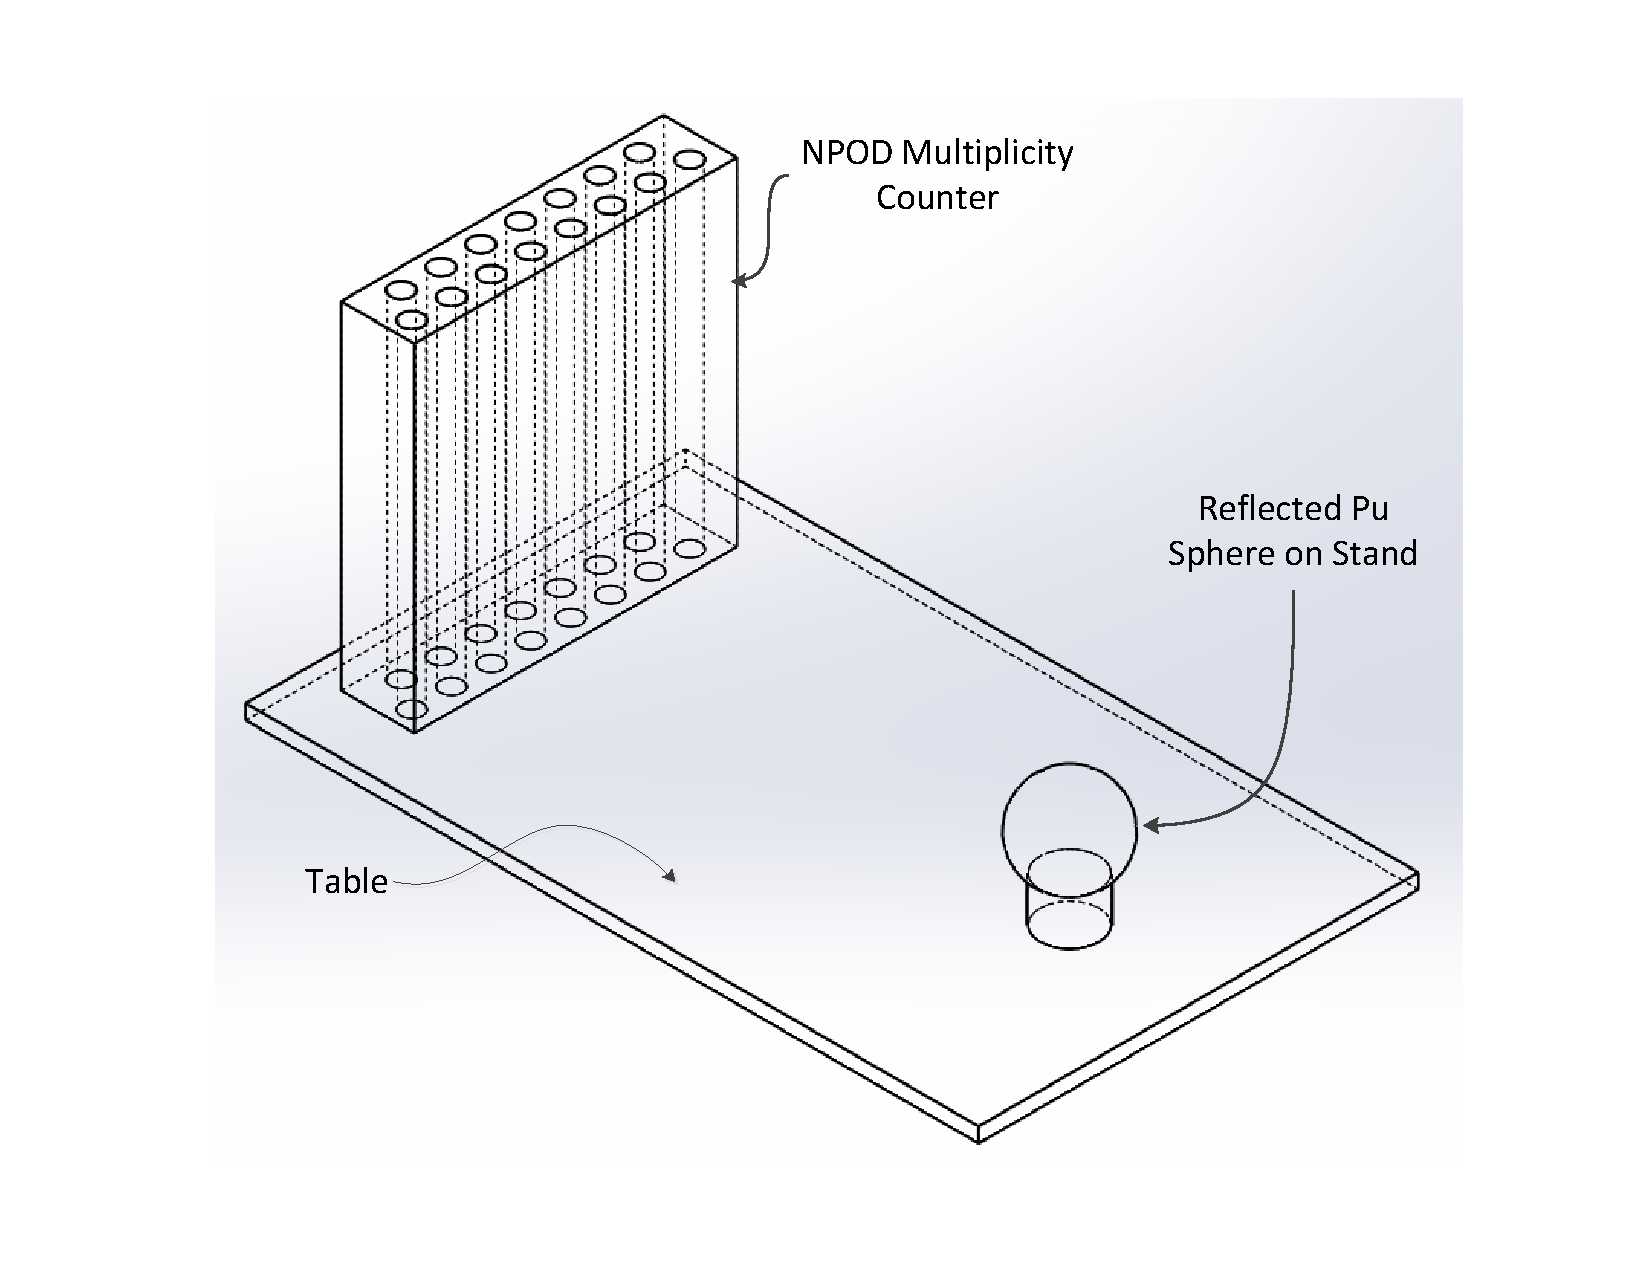
\includegraphics[trim=1.0in 0.70in 0.8in 0.50in,clip,width=1.19\textwidth]{multiplicity_experiment.pdf} \\
    {\fontsize{7pt}{6pt}\selectfont  *Not to scale}
\end{center}
\end{figure}
\end{minipage}
\begin{minipage}{0.54\linewidth}
    {\addtolength\leftmargini{-0.5in}
     \addtolength\leftmarginii{-0.2in}
     \addtolength\wideitemsep{0.1in}
\begin{itemize}
    \item[] Experimental Parameters
  \begin{itemize}
      \item 94\% \colb{\iso{Pu}{239}} sphere \vspace{-0.2in}
      \item 5 Different HDPE shells \\ \colG{From none to 3.0 cm HDPE}
  \end{itemize}
  \item[] Experiments repeated w/ \colb{\iso{Cf}{252}}
\end{itemize} 
}
\end{minipage}

\end{frame} 


\begin{frame}
    \frametitle{MCNP5 multiplicity simulations showed discrepancy \\ with experiments for
        Pu but not for \iso{Cf}{252}}
\begin{minipage}{0.41\textwidth}
\begin{figure}[ht!]
\begin{center}
	{
	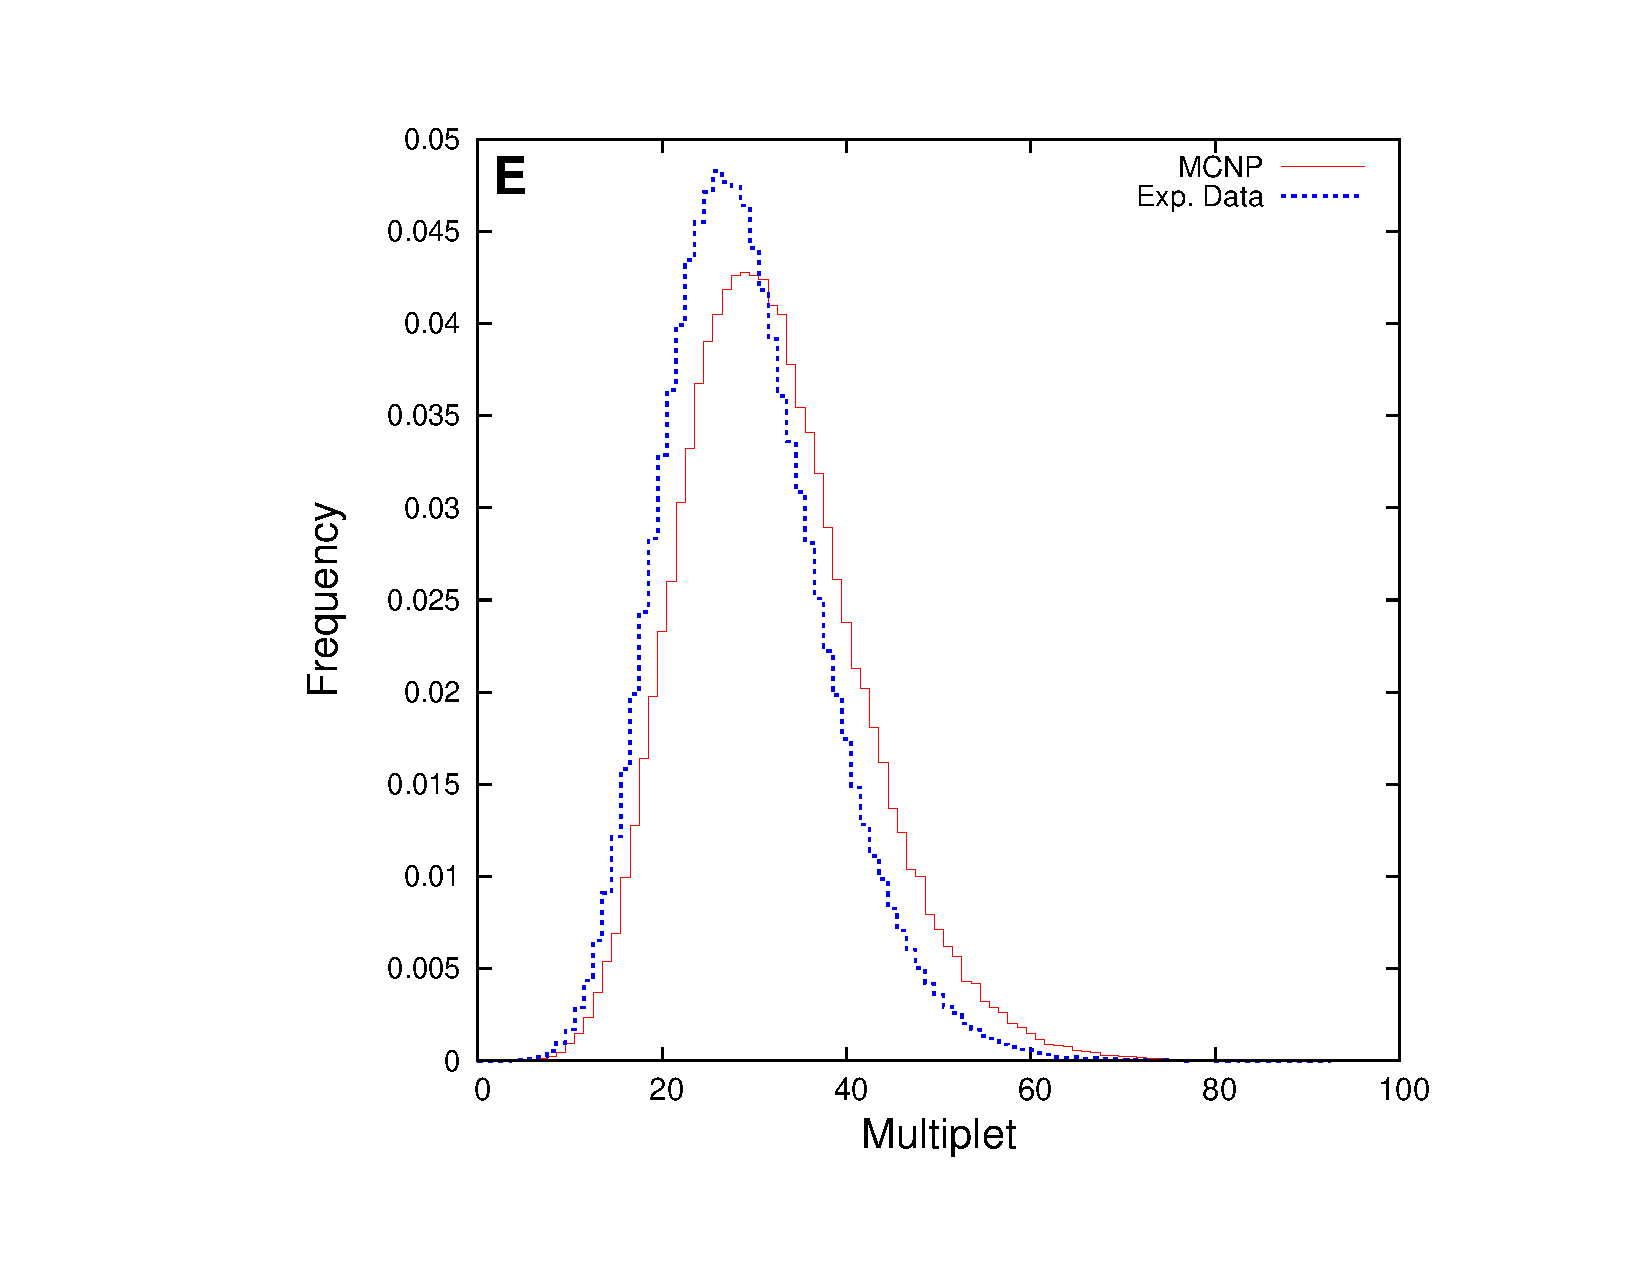
\includegraphics[trim= 2.00in 0.75in 1.450in 0.85in, clip, width=1.00\textwidth]{nubarFigures/trial_1_0_berp_3_0_2000.pdf} \\
	{\footnotesize Pu with 3.0-cm HDPE reflector} }
\end{center}
\end{figure} 
\begin{figure}[ht!]
\begin{center}
\end{center}
\end{figure} 

\end{minipage}
\begin{minipage}{0.56\textwidth}
    {\fontsize{10.8pt}{10pt}\selectfont
    \addtolength\leftmargini{-0.5in}
     \addtolength\leftmarginii{-0.2in}
     \addtolength\wideitemsep{0.1in}
\begin{itemize}
  \item[] Previous work by Mattingly [2010]
      \vspace{-0.1in}
  \begin{itemize}
      \item Caused by \textbf{\iso{Pu}{239}} \colb{nuclear data} 
	\vspace{-0.1505in}
	\item  Adjusted \colb{energy-integrated \nubar}	
	\end{itemize}
\item[]  In \textbf{ENDF-VII}, raised \nubar for \iso{Pu}{239} \\ \colG{to match \keff
    benchmarks}
    \vspace{0.1in}
  \begin{itemize}
 		\item \nubar is $\sim2\,\sigma$ \colr{above} measured data for $E < 1.5$ MeV 
	\end{itemize} 
\end{itemize} }
\end{minipage}
\end{frame} 
\begin{frame}
\frametitle{Can we reduce discrepancy in multiplicity distributions \\ without significantly
altering \keff?}
{\addtolength\leftmargini{-0.2in}
 \addtolength\wideitemsep{0.1in}
\begin{itemize}
    \item[] Perform energy-\colb{dependent} perturbations of $\overline{\nu}(E)$  in
        \iso{Pu}{239} \\ \colG{Random samples drawn from ENDF-VII.1 covariance data}
    \item[] Compare experimental and simulated multiplicity dist. 
            \\ \colG{and a $\keff$ benchmark (Jezebel)}
        \item[] Compare $\overline{\nu}(E)$ results to uniform shifts of
		microscopic cross sections 
	\end{itemize}	
}
\end{frame} 





%\section{Correlated Sampling}
%\subsection{Simulations of Multiplicity Experiments with Nuclear Data Perturbations}


%\section{Methodology}
%\subsection{Simulations of Multiplicity Experiments with Nuclear Data Perturbations}




\begin{frame}
\frametitle{We used LANL NDVV Python tools \\ to generate energy-dependent \nubar  samples}
{\addtolength\wideitemsep{0.2in}
\begin{enumerate}
	\item Generate a correlated sample of $\nubar(E)$ 
        \begin{itemize}\vspace{0.1in}
            \item {Assumed multivariate
                    Gaussian \\ \colG{ with group-averaged covariances}}
    \end{itemize}
  \item Modify continuous $\nubar(E)$ data in \textbf{ACE} file 
  \item Perform all MCNP simulations \\ \colG{with modified ACE data}
\end{enumerate} 
}
\end{frame} 



\begin{frame}
\frametitle{A cost function provides a measure \\ of inaccuracy for each data realization}
\begin{itemize}
	{
    \item[] \colb{Reduced} $\chi^2$ values for the 5 multiplicity experiments and criticality benchmark
        \begin{equation*} \hspace{0.4in}
		\begin{array}{c} 
            \displaystyle	\chi^2_{\text{red,mult,}m} = \frac{1}{N_{bins}-1}\sum_{i=1}^{N_{bins}}
	\frac{(P^{\textrm{exp}}_i - P^{\textrm{mcnp}}_i)^2}{\sigma^2(P^{\textrm{exp}}_i) + 
\sigma^2(P^{\textrm{mcnp}}_i)} 
		\end{array}
	\end{equation*} 
    \vspace{0.0in}
\item[] Equally weight $\chi^2$ values in a \colb{cost} function \\ \colG{A lower score indicatese
    higher accuracy}
	\begin{equation*}
        \boxed{\text{Cost} = \sum_{m=1}^5 \chi^2_{\text{red,mult,}m} + \chi^2_{\text{red,}\keff}}
	\end{equation*} 
}
\end{itemize}

\end{frame} 

%\begin{frame}
%\frametitle{Summary of Procedure}	
%\begin{itemize}
%	\item \colg{FOR} each \colb{trial} :
%	\begin{enumerate}
%		\item Generate a unique set of perturbed nuclear data
%		\item Run \textbf{MCNP5\_mult} simulations (5 multiplicity, \colb{JEZEBEL})
%		\item Produce multiplicity distributions
%		\item Compute $\chi^2_{red}$ values and cost
%	\end{enumerate} 
%	\item The \colb{lowest} cost is the most accurate trial
%\end{itemize}
%\end{frame} 


%\section{Results}
%\subsection{Simulations of Multiplicity Experiments with Nuclear Data Perturbations}

\begin{frame}
 \frametitle{Multiplicity and $\keff$ simulations were performed \\ for 500 unique realizations  of \nubar data}
\begin{center}
\resizebox{!}{0.5in}{
 \begin{tabular}{ccc}
	 \hline {Trial} & {Cost} & {$\chi^2_{\,{k}_{\mathrm{eff}}}$} 
\\ \hline
\nubar -1.14\%	&	164.24	&		33.66	\\	
\textbf{303}	&	\textbf{197.07}	&	\textbf{4.18}	\\	
%243	&	264.3	&	261.33	&	2.97	\\	
\colg{{55}}	&	267.9	&	\colg{0.01}	\\	
Original	&	426.86	&	0.27	\\	\hline
\end{tabular}
}
\end{center}
\begin{itemize}
    \item[]{MCNP criticality test suite performed for best data}
        \\ \colG{which includes 39 criticality benchmarks w/ \iso{Pu}{239}}:
\end{itemize}
	\begin{center}
\vspace{0.01in}
\resizebox{!}{0.50in}{
 \begin{tabular}{cc}
    \hline {Trial} & {$RMSD$} \\ \hline
\nubar -1.14\% & 1.23\% \\	
\colb{303} & \colb{0.51\%}	 \\
Original	&	0.49\% \\	\hline
\end{tabular}
}
\end{center}
\end{frame} 


\begin{frame}
\frametitle{Energy-dependent \nubar perturbations   \\ improved all 5 multiplicity
distributions}
\begin{itemize}
    \item Plots for best data realization and 3.0 cm HDPE case
\end{itemize}
\begin{center}
$\begin{array}{cc} \textbf{Original \nubar Data} & \hspace{0.13in}\textbf{Trial 303: Lowest Cost} \\
   \hspace{-0.25in}
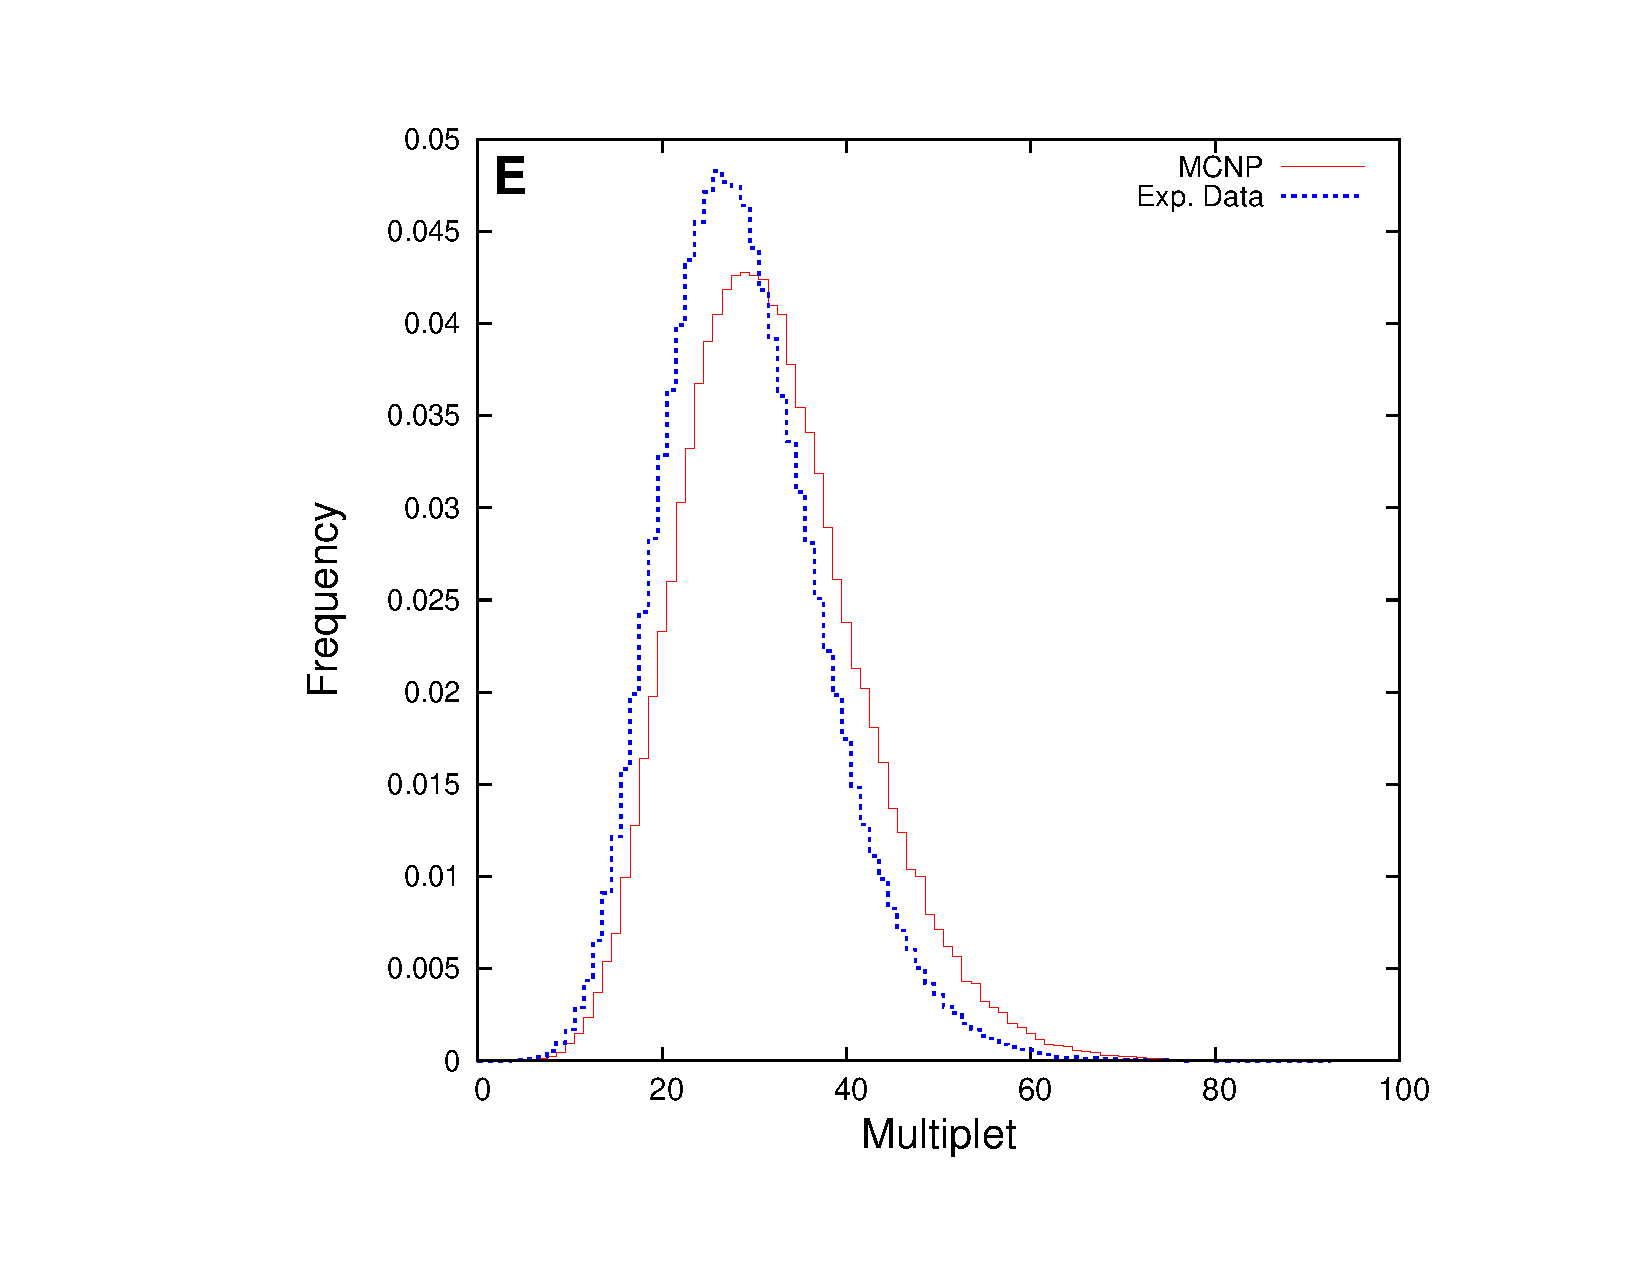
\includegraphics[trim= 1.0in 0.75in 1.0in 0.75in, clip, width=0.5\textwidth]{nubarFigures/trial_1_0_berp_3_0_2000.pdf} &
\hspace{-0.2in}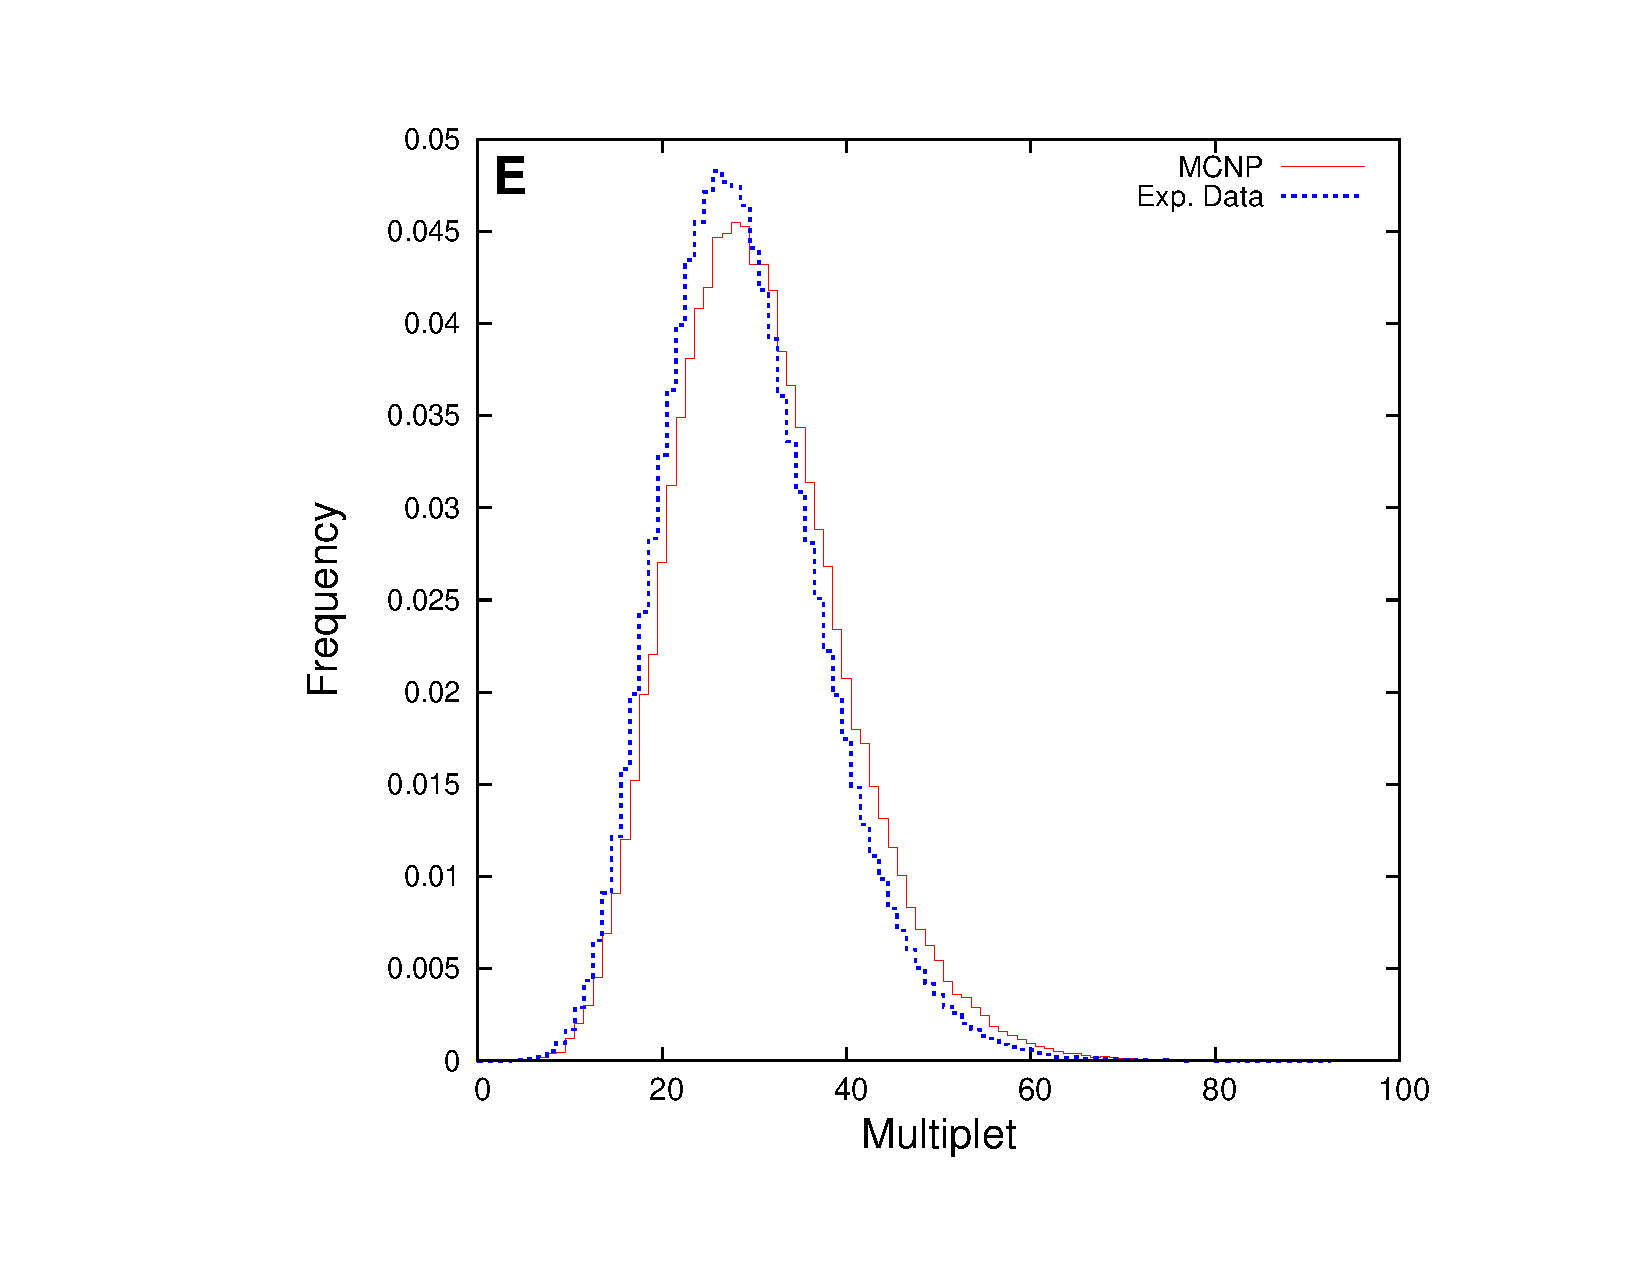
\includegraphics[trim=1.0in 0.75in  1.0in  0.75in, clip, width=0.5\textwidth]{nubarFigures/trial_303_berp_3_0_2000.pdf} \\
\end{array}$
\begin{itemize} 
	\item Best data set reduced \colb{bias} in {1$^{\text{st}}$} and {2$^{\text{nd}}$} moments, averaged over all 5 simulations, by \colb{$\sim35\%$}
\end{itemize}
\end{center}
\end{frame}


\logo{}

%\begin{frame}
%\frametitle{Capture Cross Section -- \coly{3.0 cm HDPE reflector}}
%{\small
%\begin{itemize} \vspace{-0.2in}
%	\item Adjust \colb{total cross section} ($\sigma_t$) to compensate for change in $\sigma_c$
%
%	\end{itemize} }
%	
%\begin{center}
%$\begin{array}{cc} \textbf{Original \sa Data} & \hspace{0.13in} {\sigma_c} \textbf{ increased 16\%} \\
%   \hspace{-0.25in}
%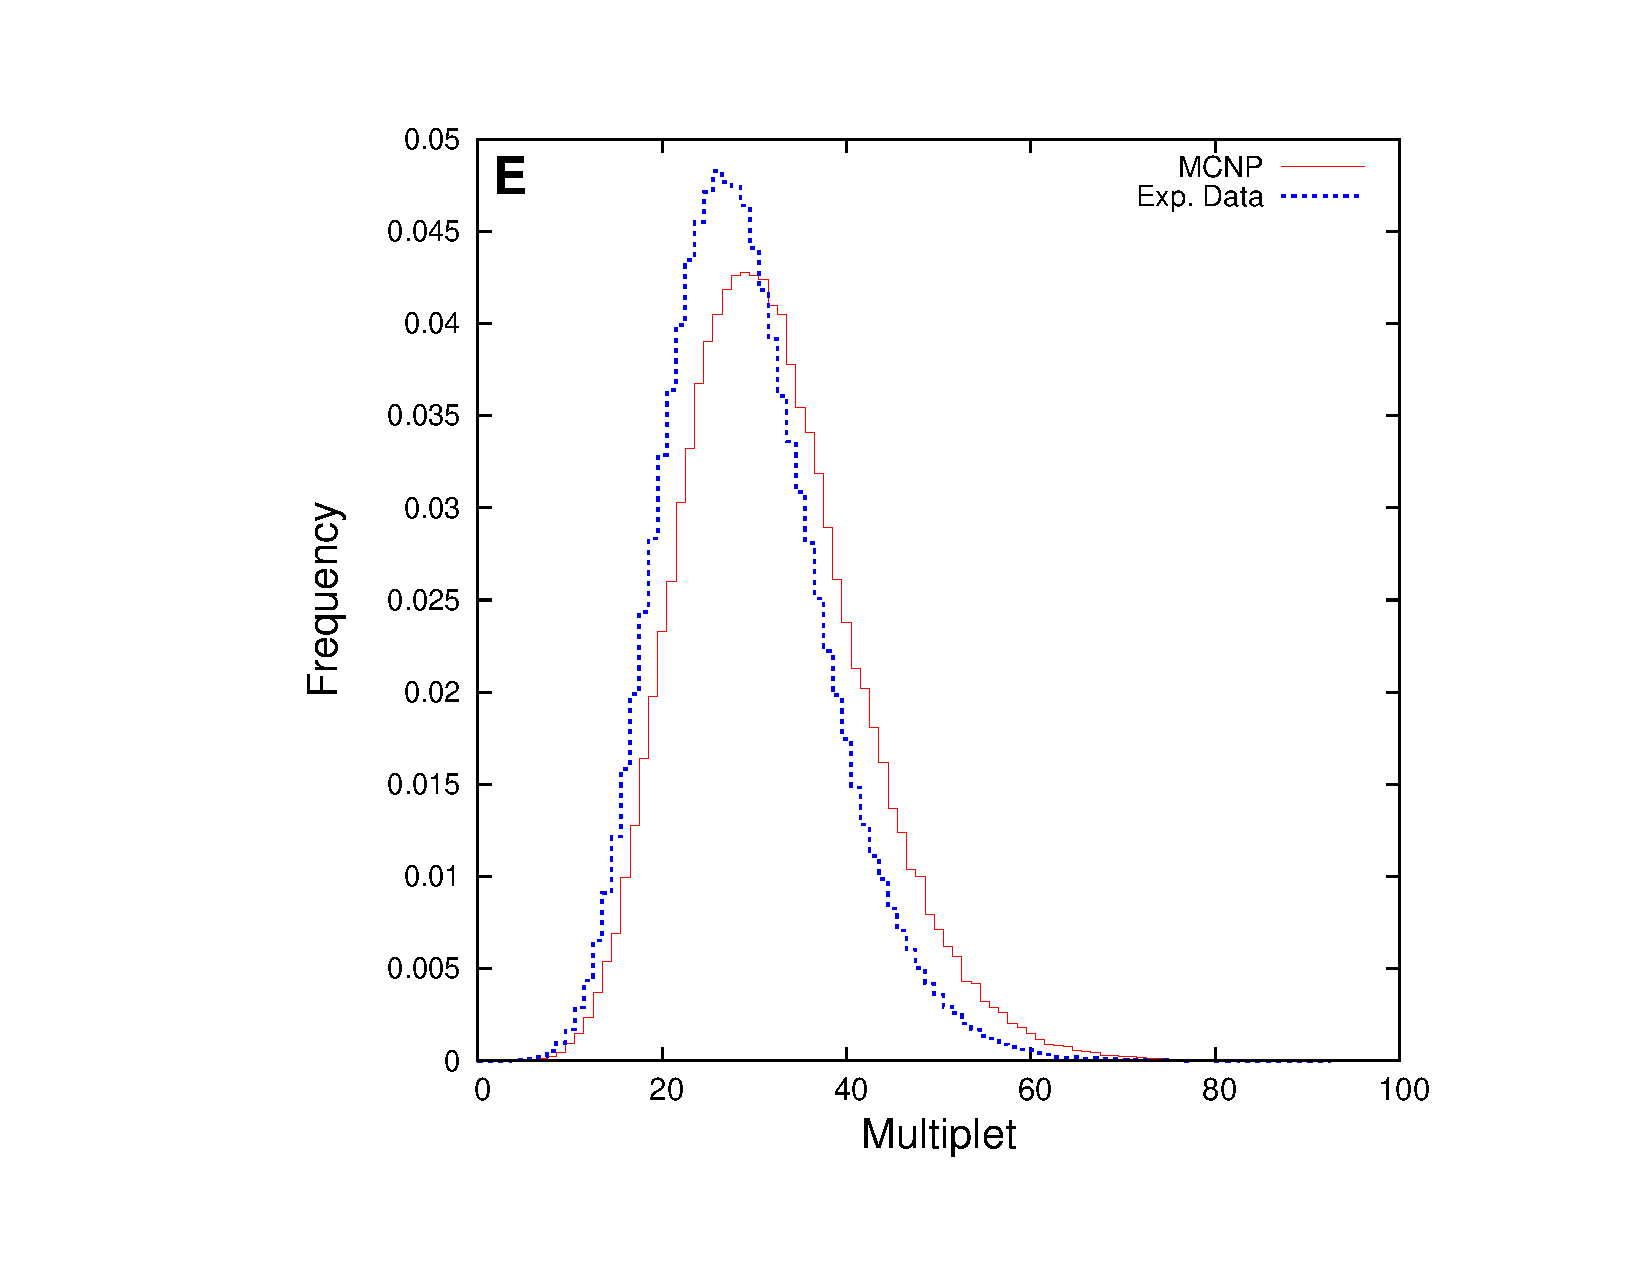
\includegraphics[trim= 1.0in 0.75in 1.0in 0.75in, clip, width=0.5\textwidth]{nubarFigures/trial_1_0_berp_3_0_2000.pdf} &
%\hspace{-0.2in}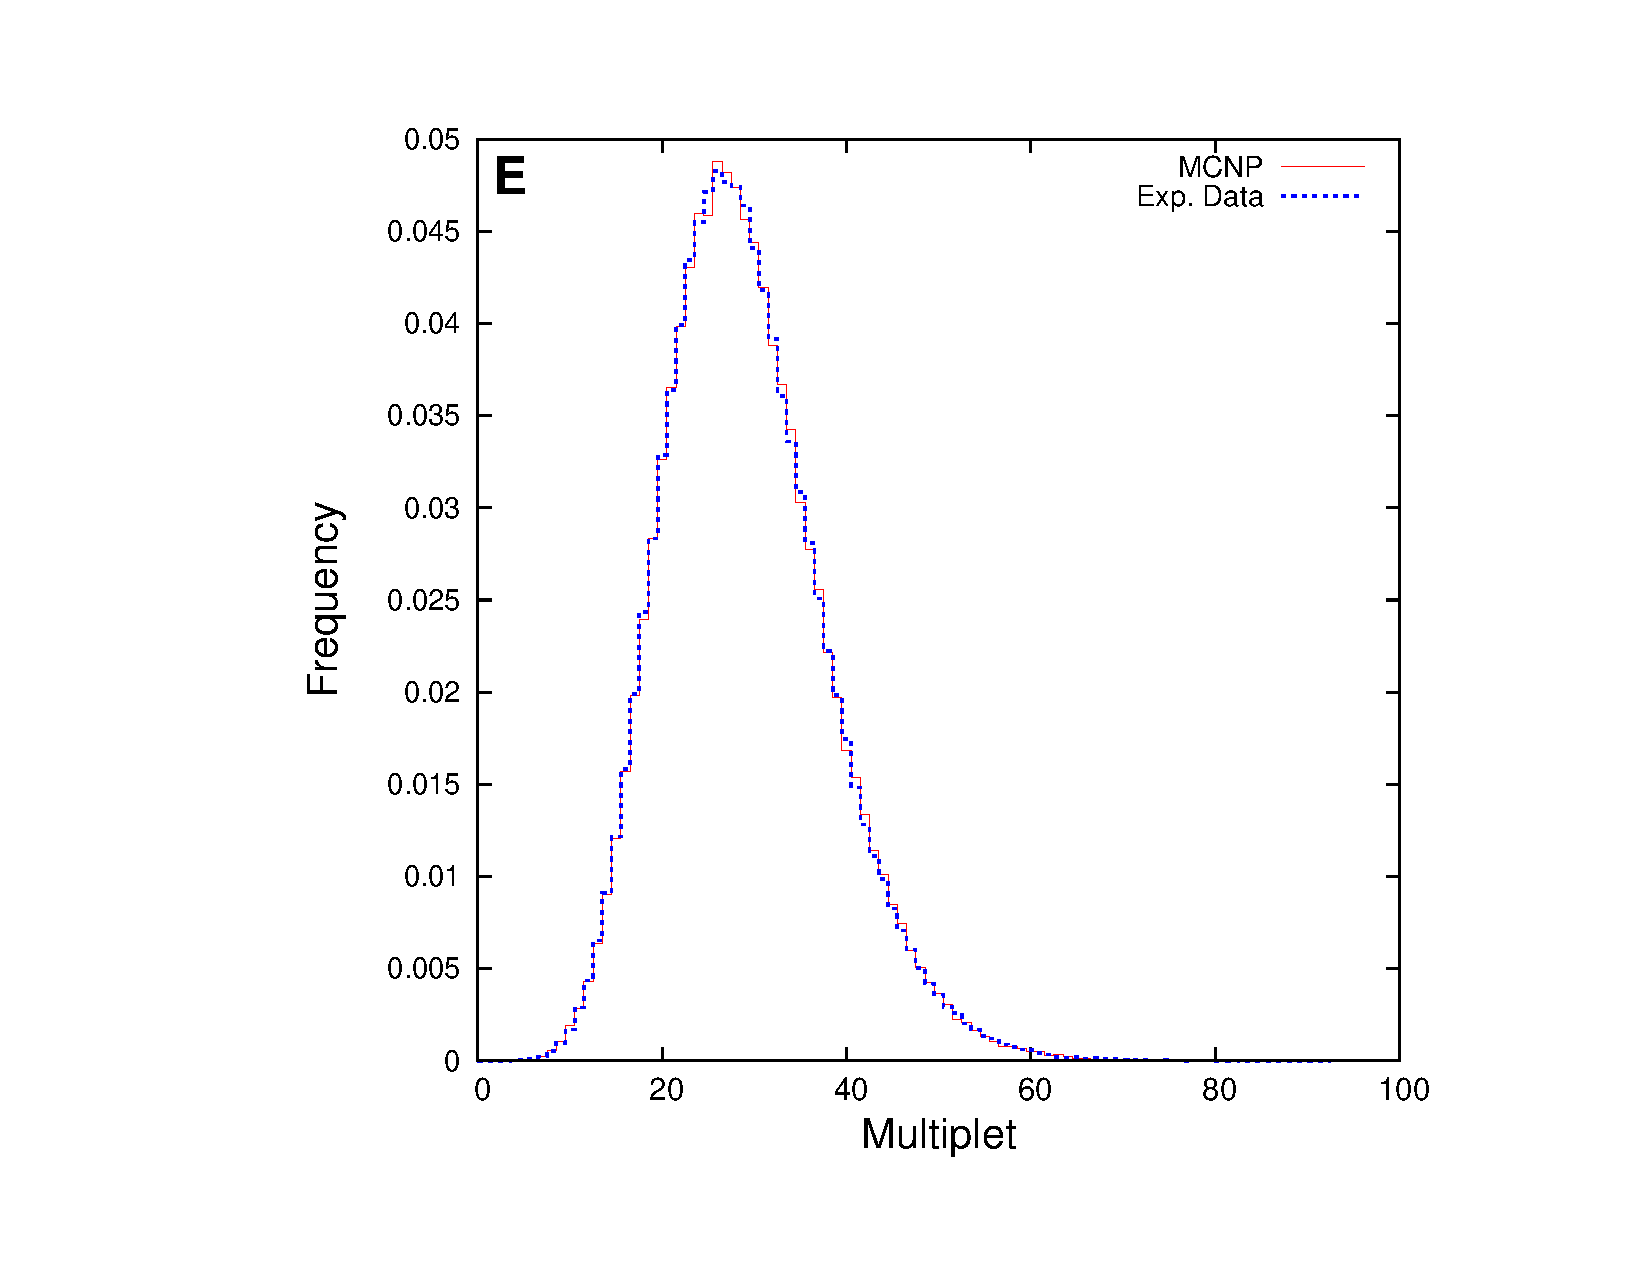
\includegraphics[trim=1.0in 0.75in  1.0in  0.75in, clip, width=0.5\textwidth]{capFigures/trial_16_0_berp_3_0_2000.pdf} \\
%\end{array}$
%\begin{itemize} 
%	\item Correction is \colr{less} for other experiments, and $\# s(\sigma_c) = \colr{7\;\sigma}$
%\end{itemize}
%\end{center}
%\end{frame}


\begin{frame}
    \frametitle{Adjusting the fission cross section \textbf{uniformly} \\ showed good correction to multiplicity
simulations}
\begin{center}
$\begin{array}{cc} \textbf{Original \sfiss Data} & \hspace{0.13in}\textbf{\sfiss decreased
    1.5\%} \\[6pt]
   \hspace{-0.25in}
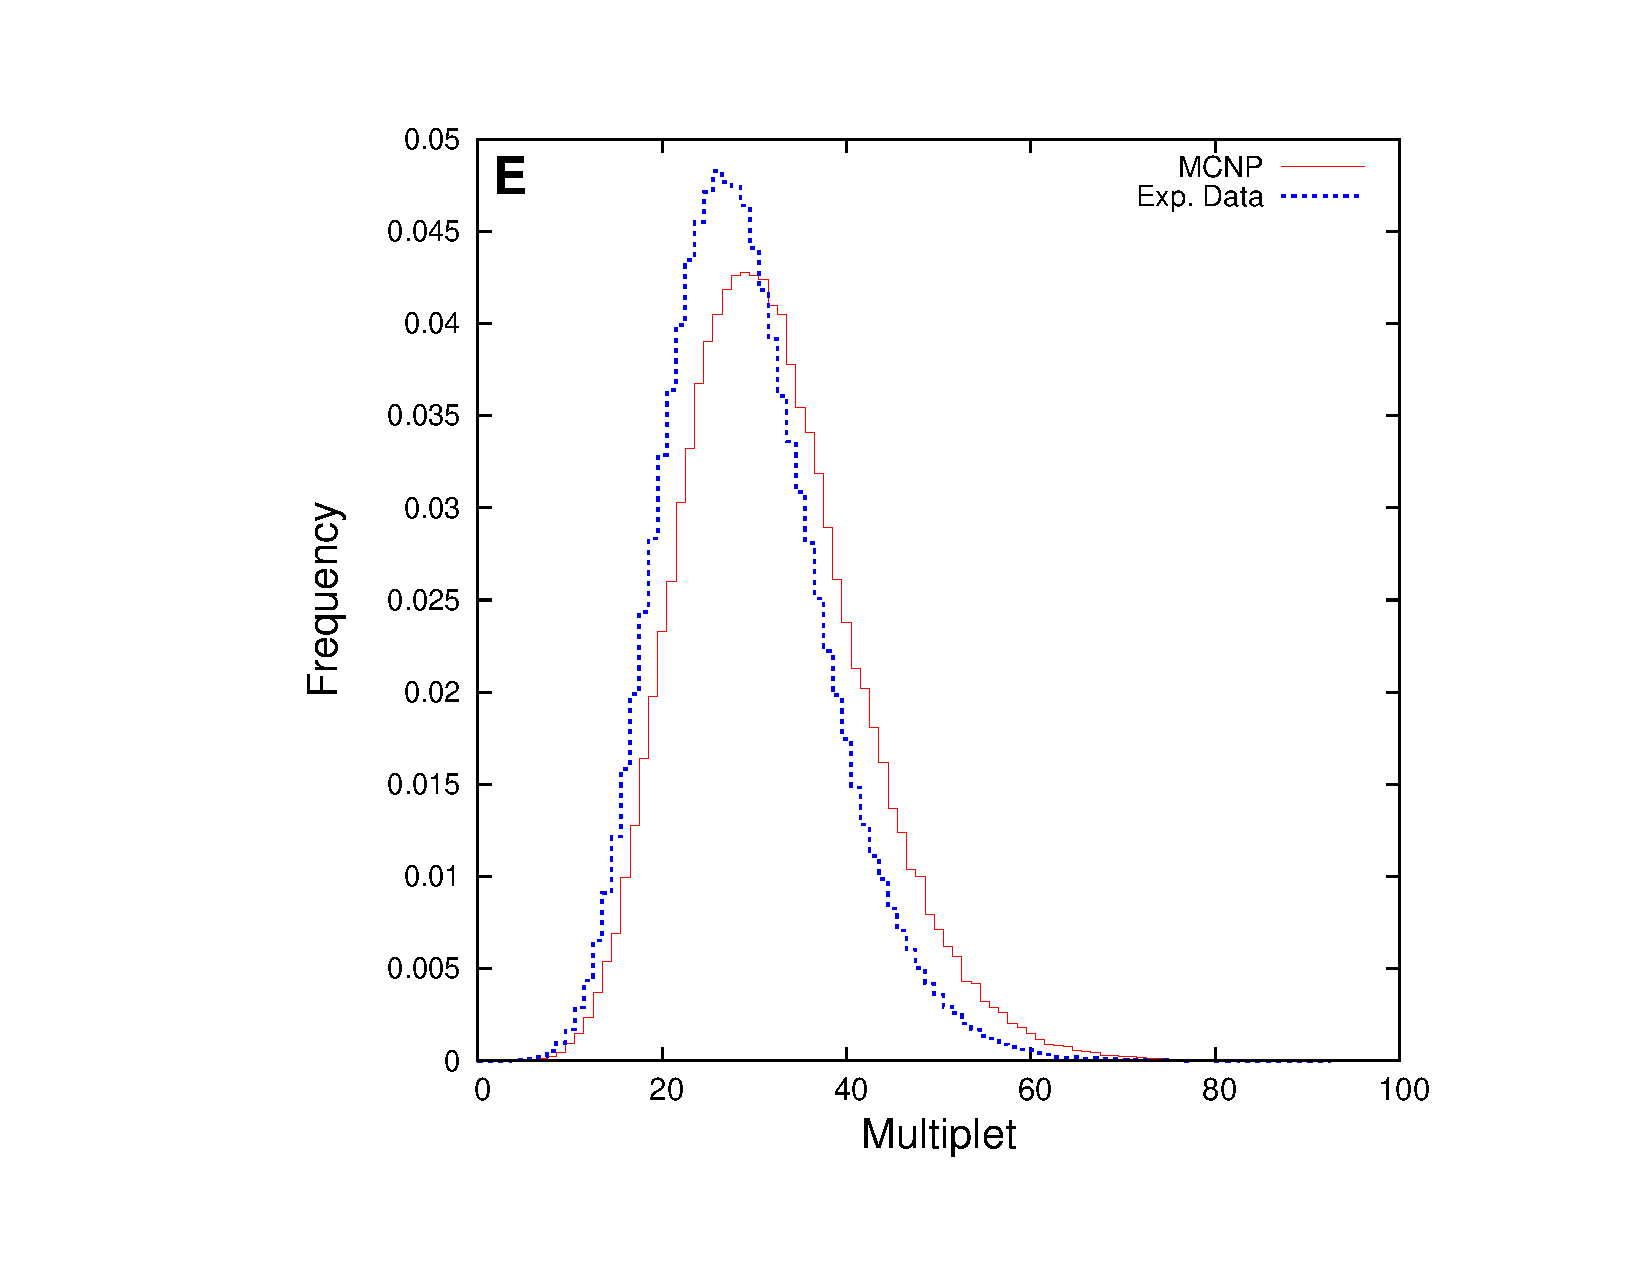
\includegraphics[trim= 1.0in 0.75in 1.0in 0.75in, clip, width=0.5\textwidth]{nubarFigures/trial_1_0_berp_3_0_2000.pdf} &
\hspace{-0.2in}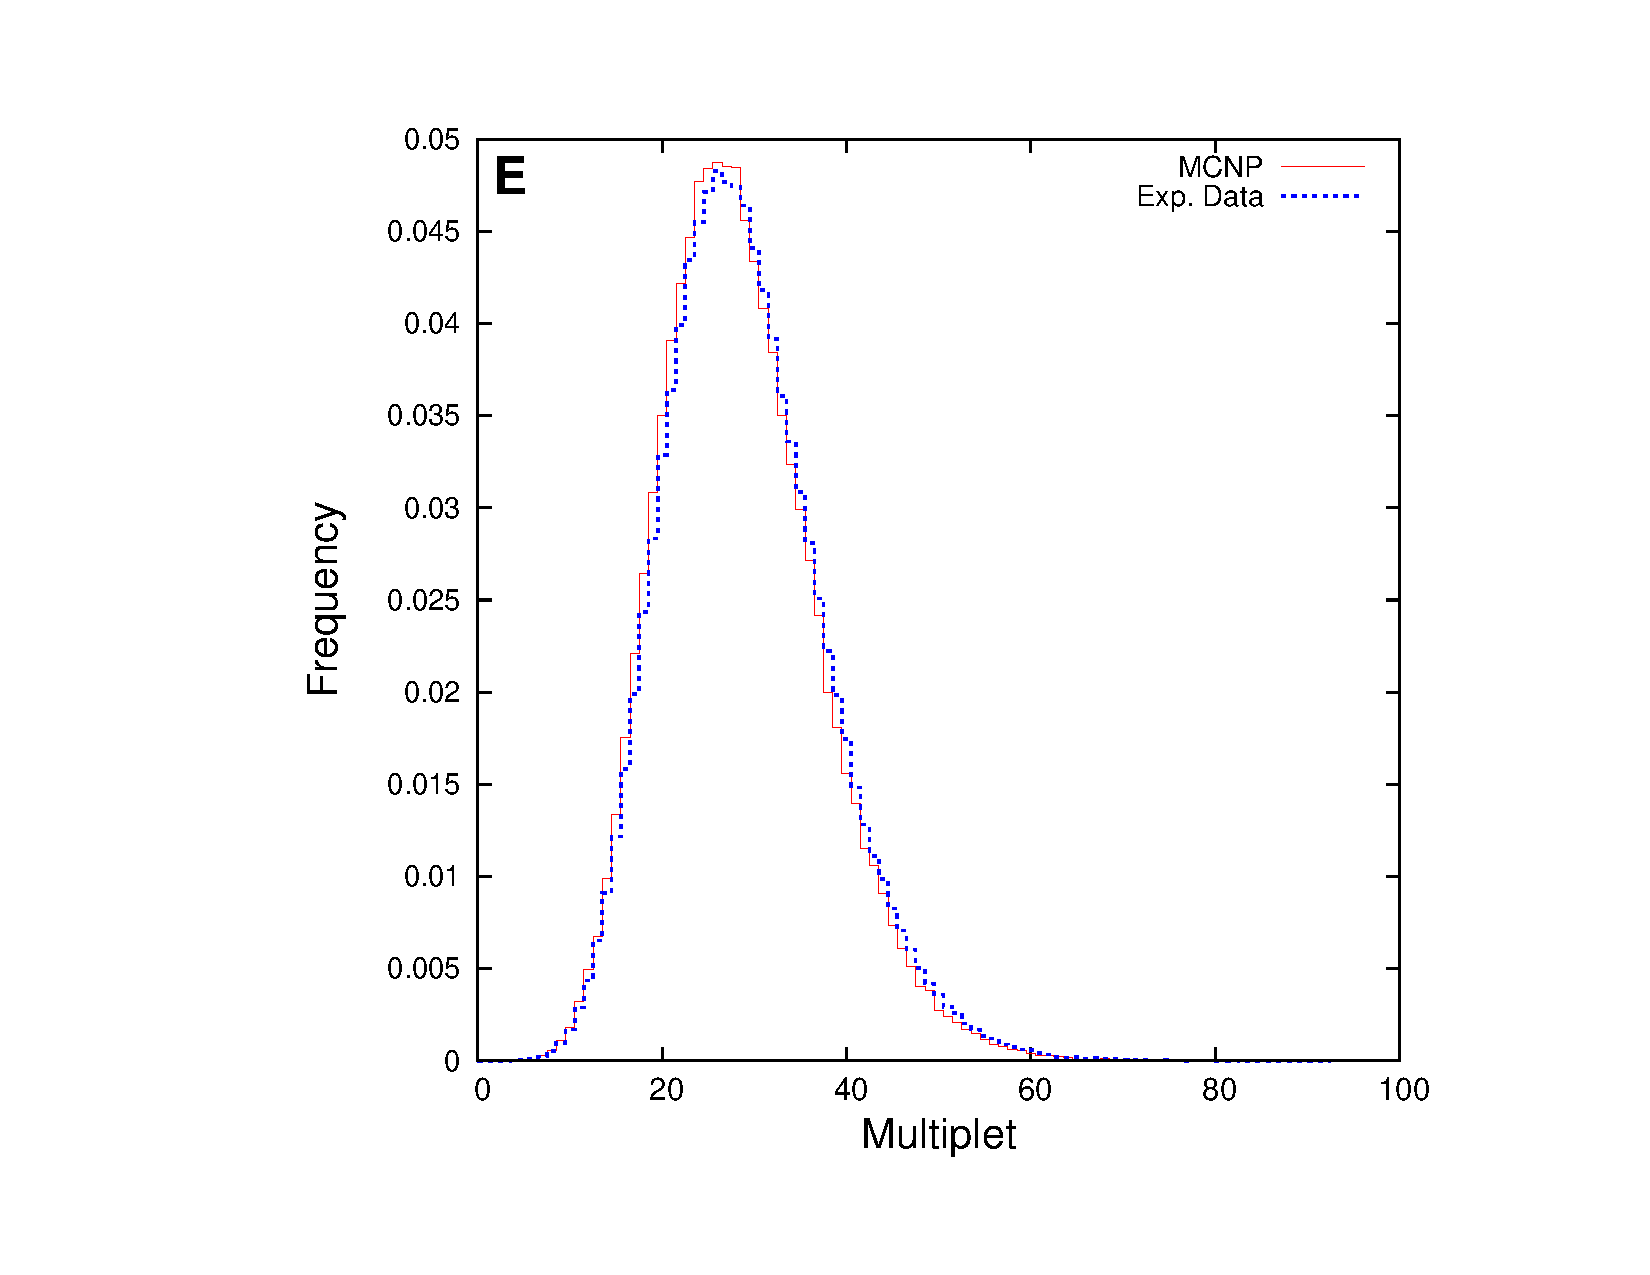
\includegraphics[trim=1.0in 0.75in  1.0in  0.75in, clip, width=0.5\textwidth]{capFigures/trial_-1_5_berp_3_0_2000.pdf} \\
\end{array}$
\end{center}
\begin{itemize} \vspace{-0.1in} 
  \item High accuracy for all simulations: $\displaystyle \sum_{i=1}^5 \chi^2_{red,mult,m} = \colb{14.6}$
      \vspace{-0.2in}
  \item \keff is \textbf{not preserved:} $\chi^2_{\keff} = 22.6$
\end{itemize} 
\end{frame}






%\section{Conclusions}
%\subsection{Simulations of Multiplicity Experiments with Nuclear Data Perturbations}
\begin{frame}
\frametitle{Simulations of Multiplicity Experiments \\ with Nuclear Data Perturbations}
	\vspace{-0.2in}
\begin{itemize}
    \item[] Energy-dependent \nubar perturbations \colb{reduced inaccuracies} in multiplicity while \colb{preserving} \keff
      \begin{itemize}\vspace{0.1in}
		\item Majority of cross-correlation terms $\mathcal{O}(10^{-4})$ or less
            \vspace{-0.1in}
        \item $\sigma_f$ may need more investigation
            \\ \colG{not sensitive to capture cross section}
	  \end{itemize}
      \item[] Subcritical simulations should be considered \\ in validation of nuclear data
      \item[] Covariance sampling methodology for nuclear data was developed and demonstrated
	\begin{itemize}
	 	\item Ideally sample all cross sections and \nubar simultaneously 

\end{itemize} 
\end{itemize}
\end{frame} 


\author{S.R. Bolding\inst{1}, \and C.J. Solomon\inst{2}}
\date{4 August 2016}
\begin{frame}
\vspace{-0.2in}
\centering
\maketitle

\end{frame} 






















